\documentclass[tikz, border=2mm]{standalone}

% Definición de colores
\definecolor{maincolor1}{RGB}{1,82,142}  % Azul oscuro
\definecolor{maincolor2}{RGB}{21,182,184} % Azul clarito

\begin{document}
	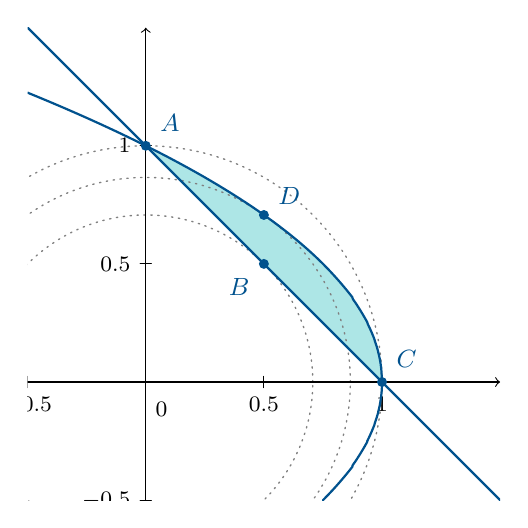
\begin{tikzpicture}[line cap=round, line join=round, x=3.0cm, y=3.0cm]
		
		% Delimitar ventana de dibujo
		\clip (-0.5, -0.5) rectangle (1.5, 1.5);
		
		% Región factible sombreada con maincolor2 (azul clarito)
		\fill [color=maincolor2, fill opacity=0.35] (1,0) -- plot[samples=500, domain=0.0:1.0] (\x, {(1-\x)^(0.5)}) -- cycle;
		
		% Curvas de nivel f(x_1, x_2) = c (Círculos concéntricos punteados)
		\draw [line width=0.5pt, dotted, color=black!50] (0,0) circle (0.707106781); % r = sqrt(0.5)  -> Mínimo B
		\draw [line width=0.5pt, dotted, color=black!50] (0,0) circle (0.866025404); % r = sqrt(0.75) -> Candidato D
		\draw [line width=0.5pt, dotted, color=black!50] (0,0) circle (1.0);         % r = 1        -> Máximos A y C
		
		% Ejes coordenados
		\draw[->, color=black] (-0.5,0.) -- (1.5,0.);
		\foreach \x in {-0.5,0.5,1}
		\draw[shift={(\x,0)}, color=black] (0pt,2pt) -- (0pt,-2pt) node[below] {\footnotesize $\x$};
		
		\draw[->, color=black] (0.,-0.5) -- (0.,1.5);
		\foreach \y in {-0.5,0.5,1}
		\draw[shift={(0,\y)}, color=black] (2pt,0pt) -- (-2pt,0pt) node[left] {\footnotesize $\y$};
		
		\draw[color=black] (0pt,-10pt) node[right] {\footnotesize $0$};
		
		% Restricción 1: x_1 + x_2 = 1 (Recta en azul oscuro)
		\draw [domain=-0.5:1.5, color=maincolor1, thick] plot(\x, {1-\x});
		
		% Restricción 2: x_1 + x_2^2 = 1 (Parábola en azul oscuro)
		\draw [samples=500, domain=-0.5:1, color=maincolor1, thick] plot(\x, {(1-\x)^(0.5)});
		\draw [samples=500, domain=0.75:1, color=maincolor1, thick] plot(\x, {-(1-\x)^(0.5)});
		
		% Puntos candidatos KKT (A, B, C, D)
		\fill [color=maincolor1] (0, 1) circle (1.8pt);
		\fill [color=maincolor1] (0.5, 0.5) circle (1.8pt);
		\fill [color=maincolor1] (1, 0) circle (1.8pt);
		\fill [color=maincolor1] (0.5, 0.707106781) circle (1.8pt);
		
		% Etiquetas de los puntos KKT
		\node [above right, color=maincolor1, font=\small\bfseries] at (0.02, 1.02) {$A$};
		\node [below left, color=maincolor1, font=\small\bfseries] at (0.48, 0.48) {$B$};
		\node [above right, color=maincolor1, font=\small\bfseries] at (1.02, 0.02) {$C$};
		\node [above right, color=maincolor1, font=\small\bfseries] at (0.52, 0.71) {$D$};
		
	\end{tikzpicture}
\end{document}